%%%%%%%%%%%%%%%%%%%%%%%%%%%%%%%%%%%%%%%%%%%%%%%%%%%%%%%%%%%
% Capitolo 4

\chapter{Tecnologie}
\label{tecnologie}





In questo capitolo verranno introdotte le principali tecnologie di 
localizzazione, di mapping e le architetture.

 RISCRIVERE!!!!







\section{Il paradigma REST}
Representational state transfer (REST)\footnote{Il paradigma REST è stato introdotto nel 2000 nella tesi di dottorato di Roy Fielding, reperibile all'indirizzo \emph{\url{http://www.ics.uci.edu/~fielding/pubs/dissertation/rest_arch_style.htm}}} è un tipo di architettura software per i sistemi di ipertesto distribuiti come il World Wide Web.
Esso si riferisce ad un insieme di principi di architetture di rete, i quali delineano come le risorse sono definite e indirizzate. Il termine è spesso usato nel senso di descrivere ogni semplice interfaccia che trasmette dati su HTTP senza un livello opzionale come SOAP o la gestione della sessione tramite i cookie.

Le applicazioni basate sui principi REST, spesso definite "RESTful", usano richieste HTTP per inviare dati (creare o aggiornare), leggere dati (eseguire query) e cancellare dati.

Nel dettaglio, lo stile architetturale di REST, rappresentato in figura \ref{restimage}, consiste di un lato client e un lato server: i client inviano richieste ai server; i server elaborano tali richieste e restituiscono ai client i risultati delle elaborazioni.
Richieste e risposte si basano sul trasferimento di rappresentazioni di \textbf{risorse}.

L'esistenza delle risorse è un concetto importante in REST, in quanto esse sono fonti di informazioni a cui si può accedere tramite un identificatore globale (un URI). Per utilizzare le risorse, le componenti di una rete (client e server) comunicano attraverso una interfaccia standard (ad es. HTTP) e si scambiano rappresentazioni di queste risorse (il documento che trasmette le informazioni).
\\
\begin{figure}[h!]
\begin{center}
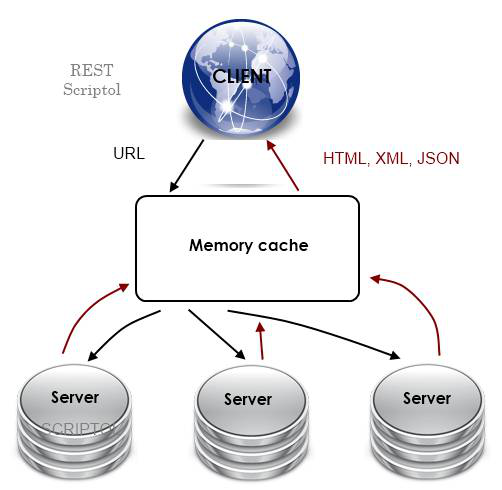
\includegraphics[scale=0.7]{imgs/rest_architecture.png} 
\caption{Modello di architettura REST\label{restimage}}
\end{center}
\end{figure}
\\
Un numero qualsiasi di connettori (client, server, cache, tunnel ecc.) può mediare la richiesta, ma ogni connettore interviene senza conoscere la “storia passata” delle altre richieste(stateless). Di conseguenza una applicazione può interagire con una risorsa conoscendo due cose: l'identificatore della risorsa e l'azione richiesta.
L'applicazione deve conoscere il formato dell'informazione (rappresentazione) restituita, tipicamente un documento HTML, XML o JSON, ma potrebbe essere anche un'immagine o qualsiasi altro contenuto.

\section{Serializzazione}
La serializzazione è un processo  per salvare un oggetto in un supporto di memorizzazione lineare o per trasmetterlo su una connessione di rete.
Essa può essere realizzata in modalità binaria o testuale.
La modalità binaria, seppur molto efficiente, presenta scarsa interoperabilità e flessibilità.
La serializzazione testuale, invece, essendo basata sulla tecnologia REST, determina un'ottimizzazione nello scambio di informazioni tra ambienti eterogenei, rendendo le strutture tradotte indipendenti dall'architettura e dalle differenti rappresentazioni dei dati.
I formati di serializzazione testuale più noti sono XML, JSON e YAML, che  sono trattati di seguito.

\subsection{XML}
La storia di XML (eXtra Markup Language)\footnote{Il formato XML è uno standard gestito dalla W3C. Il sito internet di riferimento è \emph{\url{http://www.w3.org/XML/}}} è strettamente legata a quella di SGML (Standard Generalized Markup Language), progetto ideato da IBM per migliorare l'interoperabilità aziendale, dal momento che la comunicazione tra computer era ostacolata da una ricca gamma di formati di file.

XML, infatti, è nato grazie ad una semplificazione di SGML per consentire di definire in maniera semplice nuovi linguaggi di markup da utilizzare in ambito web.
In definitiva, XML è un linguaggio marcatore basato su un meccanismo sintattico che consente di definire e controllare il significato degli elementi contenuti in un documento o in un testo.

\begin{figure}
\begin{center}
\lstset{language=MYXML}
\begin{lstlisting}
<?xml version="1.0" encoding="utf-8"?>
<!DOCTYPE Rubrica SYSTEM “Rubrica.dtd”>
<rubrica>
	<persona>
		<nome>Enrico</nome>
		<cognome>Bencivenga</cognome>
		<indirizzo>
			<via>Camillo Cucca 106</via>
			<cap>80031</cap>
			<citta>Brusciano</citta>
			<provincia>Napoli</provincia>
		</indirizzo>
	</persona>
</rubrica>

\end{lstlisting}
\caption{Esempio di documento XML\label{xmlimage}}
\end{center}
\end{figure}


\subsubsection{Sintassi}
XML è una tecnologia adoperata per creare linguaggi di markup che descrivono dati di qualsiasi tipo, quindi consente di descrivere dati in modo accurato creando nuovi tag.
Un esempio di sintassi XML è l'esempio \textbf{Rubrica.xml} della figura \ref{xmlimage}.


Un documento XML si può quindi dividere in due sezioni: il \textit{prologo} e l'\textit{istanza}. 
Il prologo contiene informazioni di carattere generale sul documento, mentre l'istanza contiene i dati. Il documento XML è costituito da un insieme di dati e di marcatori che ne specificano la struttura.
Alcuni di essi sono:
\begin{itemize}
\item Tag;
\item Processing instructions;
\item Entità;
\item Commenti;
\item Sezione CDATA.
\end{itemize}

\paragraph{Dichiarazione}
Le prime due righe contenute nell'esempio della figura \ref{xmlimage} costituiscono la dichiarazione del documento XML.
La prima riga contiene la specifica della versione di XML utilizzata e del tipo di codifica del documento. 
Nella seconda riga è stabilita la tipologia di documento alla quale appartiene il file, specificando il particolare schema DTD scelto.
La dichiarazione della tipologia di documento può essere di tre tipi:
\begin{itemize}
\item \textbf{Esterna}:
\lstset{language=MYXML}
\begin{lstlisting}
<!DOCTYPE ELEMENTO_ROOT SYSTEM "nomefile.dtd”>
\end{lstlisting}
\item \textbf{Interna}:
\begin{lstlisting}
<!DOCTYPE ELEMENTO_ROOT [CONTENUTO DTD SCHEMA]>
\end{lstlisting}
\item \textbf{Mista}:
\begin{lstlisting}
<!DOCTYPE ELEMENTO_ROOT SYSTEM "nomefile.dtd”
[CONTENUTO DTD SCHEMA]>
\end{lstlisting}
\end{itemize}

\paragraph{Tag}
L'elemento radice della figura \ref{xmlimage} è il tag \textbf{<rubrica>}, che contiene all'interno tutti gli altri elementi del documento.
Inserire più di un elemento radice è considerato errato. I tag interni sono definiti elementi \textit{child}, e sono parte dell'organizzazione gerarchica di XML.
I tag di apertura e di chiusura vanno sempre specificati, tranne nel caso non vi siano informazioni in essi. Per gli elementi vuoti XML prevede una sintassi abbreviata \textbf{<tag/>}.

\paragraph{Attributi}
I tag XML possono contenere informazioni interne che vengono definite \textit{attributi} del tag. Essi specificano proprietà intrinseche al tag e vanno indicati attraverso l'accoppiata nome-valore, come ad esempio:
\lstset{language=MYXML}
\begin{lstlisting}
<Telefono tipo="cellulare">3289196064</Telefono>
\end{lstlisting}.


\paragraph{Commenti}
Oltre alle direttive di elaborazione, in un file XML è possibile individuare i commenti, racchiusi tra le sequenze di caratteri \textbf{<!--} e \textbf{-->}. Questi possono trovarsi in qualsiasi punto del documento, ed il testo contenuto non viene elaborato dal parser.


\begin{figure}
\lstset{language=MYXML}
\begin{lstlisting}
<! ELEMENT persona (nome, cognome)>
<! ELEMENT nome (#PCDATA) >
<! ELEMENT cognome (#PCDATA) >
\end{lstlisting}
\caption{Esempio di file DTD\label{dtdimage}}
\end{figure}

\paragraph{Correttezza sintattica e validità}
Un documento XML è valido se è conforme al DTD associato.
Un DTD (Document Type Definition) è uno strumento che definisce le componenti ammesse nella costruzione di un XML. Un esempio di DTD è riportato in figura \ref{dtdimage}.





Un documento XML, in ogni caso, non deve essere necessariamente valido, ma il requisito essenziale è la correttezza nella sintassi.
Tali regole sintattiche possono essere riassunte in:
\begin{itemize}
\item Deve essere presente un solo elemento radice;
\item I tag non possono iniziare con numeri o caratteri speciali e contenere spazi;
\item I tag devono essere innestati correttamente;
\item Tutti i tag e gli attributi sono espressi in minuscolo;
\item E' obbligatorio inserire i tag di chiusura, sia in forma estesa che in forma abbreviata, ove consentito.
\end{itemize}
Se un documento è sintatticamente valido, può essere analizzato da un \textit{parser}, un programma che, analizzando la struttura grammaticale del documento XML, ne ricostruisce l'albero a partire dall'elemento radice e proseguendo con gli elementi child.


\subsection{JSON}
JSON (JavaScript Object Notation) è un formato di serializzazione nato appositamente per lo scambio dei dati.
Un documento JSON è di facile interpretazione anche senza il processo di parsing, data la leggibilità della sua struttura.

JSON è completamente indipendente dal linguaggio di programmazione utilizzato, in quanto utilizza convenzioni conosciute dai programmatori di linguaggi della famiglia del C. 
Grazie a queste caratteristiche, JSON è un linguaggio ideale per lo scambio dei dati e per l'interoperabilità.
Con JSON è possibile rappresentare quattro tipi primitivi:
\begin{itemize}
\item numeri;
\item stringhe;
\item variabili booleane;
\item NULL.
\end{itemize}
e due tipi strutturati:
\begin{itemize}
\item array;
\item oggetti.
\end{itemize}

Il formato JSON è ampiamente diffuso, soprattutto tra gli sviluppatori web, per le dimensioni inferiori dello stream dati, dovute alla sua bassa ridondanza.

\subsubsection{Sintassi}
La sintassi JSON è molto semplice e si basa su due strutture:
\begin{itemize}
\item \textbf{coppia nome/valore}, realizzabile in diversi linguaggi di programmazione come un oggetto, un record, uno struct, una tabella hash, un elenco di chiavi o un array associativo;
\item \textbf{elenco ordinato di valori}, realizzabile nella maggior parte dei linguaggi di programmazione con un array, un vettore, un elenco o una sequenza.
\end{itemize}
Queste due strutture sono utilizzabili in tutti i linguaggi di programmazione, e ciò rende ancora più evidente la natura di JSON, orientata all'interoperabilità.

\begin{figure}
\lstset{language=JSON}
\begin{lstlisting}
{"nome": "enrico"}
\end{lstlisting}
\caption{Esempio di oggetto JSON\label{jsonobjectimage}}
\end{figure}
\paragraph{Oggetto}
Un oggetto in JSON è contenuto tra due parentesi graffe. Tra il nome e il valore sono presenti due punti ed il nome dell'oggetto è scritto tra due doppi apici, mentre il valore è scritto tra due doppi apici nel caso non sia numerico. Un esempio è in figura\ref{jsonobjectimage}.

\begin{figure}
\lstset{language=JSON}
\begin{lstlisting}
{"serializzazione": ["XML", "JSON", "altro"]}
\end{lstlisting}
\caption{Esempio di oggetto JSON\label{jsonarrayimage}}
\end{figure}

\paragraph{Array}
Un array è una raccolta ordinata di valori. In JSON un array è contenuto tra due parentesi quadre e i valori sono separati da virgola, come è evidente dalla figura \ref{jsonarrayimage}.

Le stringhe sono rappresentate come nella maggior parte dei linguaggi di programmazione e vanno sempre messe tra doppi apici, mentre i numeri possono iniziare con identificatori di segno ed essere seguiti da una parte esponenziale, così come in molti linguaggi.
Solo le rappresentazioni esadecimali o ottali non sono permesse.
\begin{figure}
\lstset{language=JSON}
\begin{lstlisting}
{
  "rubrica": {
    "persona": {
      "nome": "Enrico",
      "cognome": "Bencivenga",
      "indirizzo": {
        "via": "Camillo Cucca 106",
        "cap": "80031",
        "citta": "Brusciano",
        "provincia": "Napoli"
      }
    }
  }
}
\end{lstlisting}
\caption{Esempio di oggetto JSON\label{jsonimage}}
\end{figure}

Nell'immagine \ref{jsonimage} è possibile visualizzare un esempio completo di file JSON, analogo a quello precedente di file XML in figura \ref{xmlimage}.
L'indentazione è utilizzata solo a scopo di chiarezza sintattica, ma il testo si estende su di una sola riga, senza caratteri di ritorno a capo.
Naturalmente anche un documento JSON può essere elaborato da un parser e ricostruito.

\subsection{YAML}
YAML (YAML Ain't Markup Language), sito web di riferimento \emph{\url{http://yaml.org}}, è un linguaggio nato nel 2001 con l'obiettivo di essere \textit{human-friendly}.
E' progettato per persone che lavorano con dati, grazie alla sua comprensibilità ed interoperabilità.
YAML è peraltro un linguaggio molto pulito, in quanto riduce al minimo la quantità di caratteri strutturali e permette di mostrare i dati in modo naturale e significativo.
Gli obiettivi di YAML sono:
\begin{itemize}
\item semplicità di lettura;
\item corrispondenza con i tipi per la maggioranza dei linguaggi di programmazione;
\item esportabilità dei dati;
\item estendibilità;
\item facilità di implementazione e usabilità.
\end{itemize}

\subsubsection{Sintassi}
YAML mette a disposizione due tipi di sintassi, una indentata e una in linea, simile al formato JSON.
Inoltre in YAML ci sono degli indicatori che servono a descrivere la struttura ed il contenuto di un documento YAML.

\begin{figure}
\lstset{language=YAML}
\begin{lstlisting}
--- # Discipline
 - Matematica
 - Informatica
 - Fisica
\end{lstlisting}
\caption{Lista nel formato indentato YAML\label{yamllistaimage}}
\end{figure}

\begin{figure}
\lstset{language=YAML}
\begin{lstlisting}
 --- # Discipline
 [Matematica, Informatica, Fisica]
\end{lstlisting}
\caption{Lista nel formato convenzionale YAML\label{yamllistbimage}}
\end{figure}

\begin{figure}
\lstset{language=YAML}
\begin{lstlisting}
--- # Blocco indentato
   nome: Enrico Bencivenga
   eta: 30
 --- # Blocco allineato
 {nome: Enrico Bencivenga, eta: 30}
\end{lstlisting}
\caption{Array in YAML\label{yamlarrayimage}}
\end{figure}

\begin{figure}
\lstset{language=YAML}
\begin{lstlisting}
 --- |
	Questa è la 
		tesi di laurea
			in Ingegneria Informatica
		di Enrico Bencivenga
	matr. 534000442
\end{lstlisting}
\caption{Stringa nel formato indentato YAML\label{yamlstringaimage}}
\end{figure}

\begin{figure}
\lstset{language=YAML}
\begin{lstlisting}
 --- >
Questa è la 
tesi di laurea
in Ingegneria Informatica
di Enrico Bencivenga
matr. 534000442
\end{lstlisting}
\caption{Stringa nel formato convenzionale YAML\label{yamlstringbimage}}
\end{figure}

\paragraph{Liste}
Le liste sono collezioni di elementi. La loro rappresentazione in YAML può essere indentata (fig. \ref{yamllistaimage}) o allineata (fig. \ref{yamllistbimage}).

\paragraph{Array associativi}
Gli array sono associazioni nome/valore, e possono essere rappresentati come in figura \ref{yamlarrayimage}.

\paragraph{Stringhe}
Le stringhe non richiedono gli apici o i doppi apici per essere rappresentate.

La rappresentazione delle stringhe può essere indentata, come nella figura \ref{yamlstringaimage}, oppure allineata, come nella figura \ref{yamlstringbimage}, dove il testo viene allineato in un singolo paragrafo.

\subsubsection{Confronto tra XML, JSON e YAML}
JSON è caratterizzato dalla semplicità di rappresentazione delle strutture dati e da una bassa ridondanza, dovuta all'assenza dei tag di chiusura; è molto facile da interpretare e per questo si adatta alle applicazioni web-based.\\

YAML ha caratteristiche aggiuntive rispetto a JSON, quali l'estensibilità dei tipi, la rappresentazione di stringhe senza apici, gli anchors e gli aliases. Anche YAML risulta molto adatto alle applicazioni web-based.\\
XML ha più vincoli di YAML e JSON, poichè è nato per essere compatibile con SGML, ma risulta più adatto alla descrizione di strutture dati e presenta uno spettro di utilizzo più vasto.




\section{Geolocalizzazione}
La geolocalizzazione è l'identificazione della posizione geografica di un dato oggetto nel mondo reale.
Gli oggetti possono essere telefoni cellulari, pc, tablet, palmari e ci sono diverse tecniche, indoor ed outdoor.
\begin{itemize}
\item \textbf{outdoor}: localizzazione satellitare;
\item \textbf{indoor}: infrastrutture ad-hoc e WiFI;
\item \textbf{indoor ed outdoor}: infrastruttura cellulare.
\end{itemize}
Vi sono inolte diversi metodi per valutare la qualità di un sistema di localizzazione:
\begin{itemize}
\item \textbf{Errore medio}: corrispondenza tra la posizione stimata e quella reale;
\item \textbf{Probabilità di corretta locazione}: probabilità di localizzare l'obiettivo entro una determinata soglia;
\item \textbf{Rendimento}: capacità del metodo a stimare la posizione in tutti i tipi di ambienti;
\item \textbf{Consistenza}: misura della stabilità dell'errore medio in ambienti differenti;
\item \textbf{Overhead}: quantità di informazione scambiata tra il terminale ed il sistema;
\item \textbf{Consumo di potenza}: quantita delle risorse energetiche impiegate;
\item \textbf{Latenza}: intervallo di tempo tra la richiesta di posizionamento e la risposta del sistema;
\item \textbf{Costi roll-out}: costi necessari all'installazione dell'infrastruttura;
\item \textbf{Costi operativi}: costi legati al mantenimento dell'infrastruttura.
\end{itemize}

\subsection{Localizzazione satellitare}
La localizzazione satellitare si basa su infrastrutture indipendenti dedicate, ovvero un certo numero di satelliti utilizzati solo a questo scopo e di tipo terminal-based.
I vantaggi del posizionamento satellitare sono la copertura globale e l'alto livello di accuratezza, ma è soggetto anche ad importanti inconvenienti, come un eccessivo consumo dovuto ai dispositivi che utilizzano il segnale GPS e ai disturbi naturali che possono ostacolarne la ricezione.

\subsubsection{GPS}
Il sistema GPS (Global Positioning System)\footnote{Il sito di riferimento per lo standard GPS è \emph{\url{http://www.gps.gov}}.}, avviato dagli USA negli anni '70 e completato nel 1993, è stato realizzato per motivi essenzialmente militari, al fine di consentire il percorso dei mezzi militari, sia sulla terraferma che in mare in modo da localizzarne la posizione in ogni momento e consentire eventuali operazioni di supporto e salvataggio.
Il GPS utilizza dai 24 ai 32 satelliti artificiali, divisi in gruppi da 4, che ruotano attorno alla terra a circa 20.200 km in orbite che formano tra loro angoli di 60 gradi.

\begin{figure}
\begin{center}

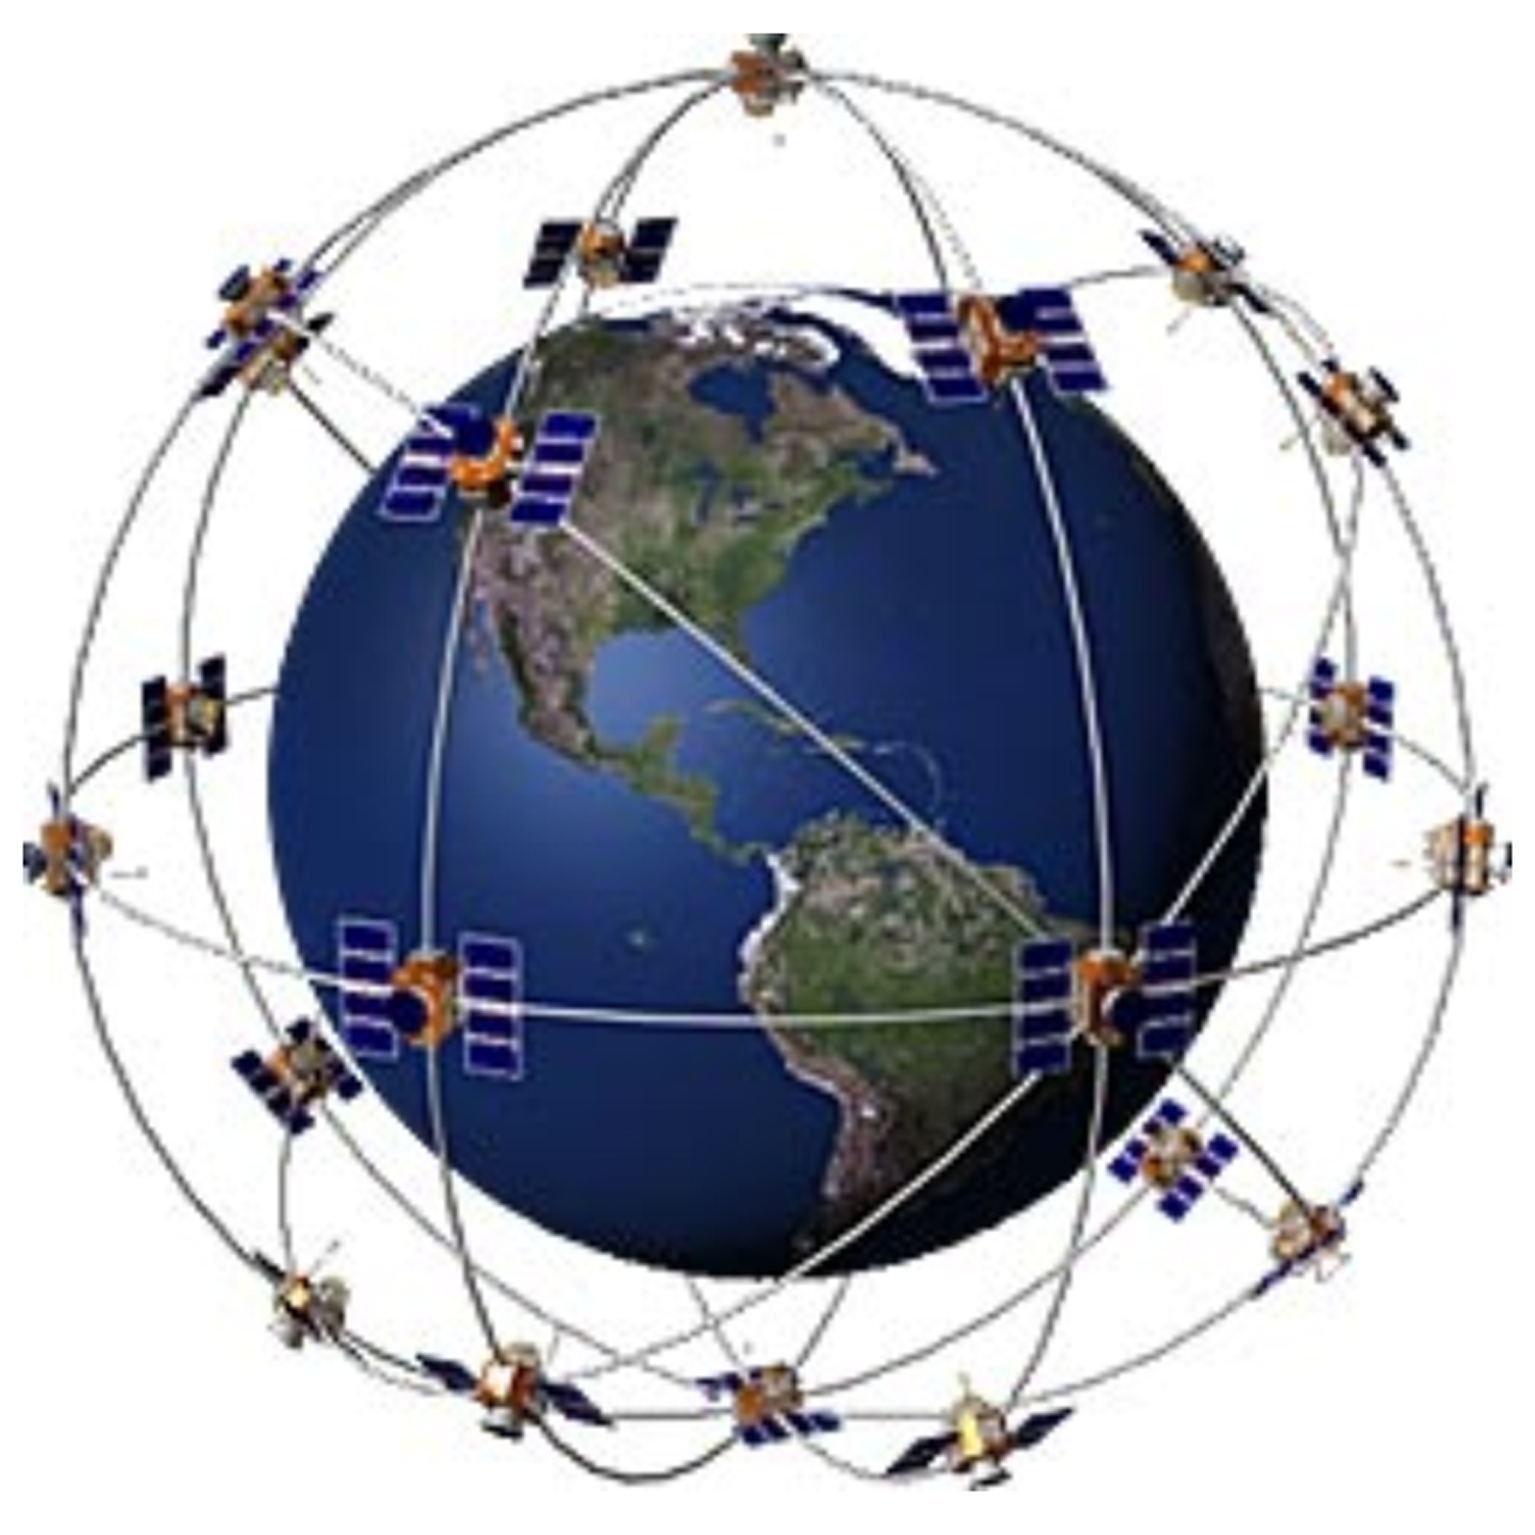
\includegraphics[scale=0.3]{imgs/gpssatelliteimage.jpg}
\caption{Rappresentazione dei satelliti GPS in orbita intorno alla terra\label{gpsimage}}
\end{center}

\end{figure}

\paragraph{Principi di funzionamento}
Il sistema GPS è nato come versione satellitare e perfezionamento del sistema LORAN, nato negli USA attorno al 1940, che consentiva la determinazione della posizione lungo le rotte di grande traffico navale ed aereo, utilizzando un grande numero di stazioni terrestri.

Il sistema GPS, così come il LORAN, consente di determinare la propria posizione sulla superficie terrestre e la propria altitudine in qualunque punto ci si trovi tramite un ricevitore GPS, il quale intercetta a terra il segnale generato dai satelliti in orbita che passano sopra di noi, così come rappresentato in figura \ref{gpsimage}.
Infatti, visto il numero, l'orbita ed il periodo di rotazione, in ogni istante e in ogni punto terreste è possibile intercettare il segnale generato da 6 a 12 satelliti.

\paragraph{Satelliti}
Le funzioni dei satelliti possono essere così sintetizzate:
\begin{itemize}
\item trasmettere informazioni agli utilizzatori mediante un segnale radio;
\item mantenere un riferimento di tempo accurato, grazie agli orologi di bordo;
\item ricevere e memorizzare informazioni dal segmento di controllo;
\item eseguire manovre e correzioni di orbita.
\end{itemize}

\paragraph{Ricevitore}
I ricevitori GPS commerciali, dal costo molto contenuto, consentono di sintonizzarsi automaticamente sulle frequenze dei satelliti GPS e, dopo un tempo di ricerca relativamente breve, di determinare la propria posizione ed, eventualmente, la propria quota, elaborando le distanze di almeno quattro satelliti.
Nei navigatori GPS per auto e negli smartphone, il risultato dell'elaborazione viene mostrato come punto all'interno di una cartina geografica completa, che può essere ingrandita fino a diventare una vera e propria cartina topografica.

\paragraph{Precisione}
La precisione della ricezione GPS è influenzata da una serie di fattori, tra cui la posizione dei satelliti, l'eventuale presenza di rumore del segnale radio, le condizioni atmosferiche e le barriere naturali.
In generale, tali disturbi possono introdurre errori di precisione tra 1 e 10 metri.
La determinazione  più accurata della  posizione si verifica quando il satellite e il ricevitore GPS sono in vista tra loro senza  nessun altro oggetto schermante. Sotto questa ipotesi, il margine di errore del posizionamento è di circa 90 cm.

\subsection{Localizzazione cellulare}
La localizzazione cellulare è utilizzata nelle reti cellulari, come GSM o UMTS, per ricavare la posizione di un utente.
Questo sistema di localizzazione è utilizzato per ricavare la presenza di un utente all'interno di una cella, per cui è soggetto a margini di errore abbastanza ampi.
Per questo motivo, i gestori hanno predisposto nuovi strumenti per equipaggiare le proprie reti con dispositivi e protocolli finalizzati alla realizzazione del posizionamento in modo più accurato ed efficiente.
A tal proposito, diversi metodi sono stati specificati dai gruppi di standardizzazione, come 3GPP (\emph{\url{http://www.3gpp.org}}. La maggior parte di questi metodi è network-based, per cui anche i dispositivi più datati possono usufruirne.
Il vantaggio di questi sistemi di localizzazione cellulare è che possono essere utilizzati anche in ambienti chiusi, diversamente dai sistemi satellitari.
Il posizionamento cellulare può essere molto costoso per quanto riguarda l'overhead dovuto alla segnalazione, soprattutto se è richiesto un alto grado  di accuratezza e, inoltre, la capacità impiegata per la localizzazione è indisponibile per i servizi voce e dati.

\subsection{Localizzazione indoor}
La localizzazione indoor è nata per essere utilizzata all'interno di grandi edifici, campus universitari, strutture museali, strutture ospedaliere e uffici di vario genere.
E' basata su tecnologie radio, infrarossi o ad ultrasuoni, con un raggio di comunicazione evidentemente limitato.
La realizzazione di un sistema di localizzazione indoor può avvenire mediante la realizzazione di infrastrutture dedicate o l'utilizzo di infrastrutture preesistenti, come le reti WLAN.
La localizzazione indoor ha il vantaggio di presentare un basso consumo di potenza dei dispositivi utilizzati per la ricezione e l'elevata accuratezza dovuta al corto raggio delle tecnologie usate.

Esistono diverse soluzioni commerciali per la localizzazione indoor, come \textbf{RADAR} (\emph{\url{http://research.microsoft.com/en-us/projects/radar/}}), sviluppata da Microsoft, che è un sistema a radio frequenza; \textbf{Real Time Location System - RTLS} (\emph{\url{http://www.ekahau.com/real-time-location-system/technology}}), di Ekahau, che si basa sull'infrastruttura WLAN IEEE 802.11; \textbf{Visibility System} (\emph{\url{http://www.aeroscout.com/technology}}), di Aeroscout, basato sempre sull'infrastruttura WLAN IEEE 802.11; \textbf{Wireless Location Appliance} (\emph{\url{http://www.cisco.com/en/US/products/ps6386/index.html}}), di Cisco, basato su WLAN.\\


\section{Web Mapping}
Il Web Mapping è un processo di progettazione, implementazione, generazione e produzione di mappe sul web.
Un caso particolare di mappe web sono le mappe mobili, visualizzate su periferiche mobili, come telefonini, smartphone, tablet e GPS.

I vantaggi derivanti dall'utilizzo di mappe web sono:
\begin{itemize}
\item facilità di generazione di mappe aggiornate;
\item economicità dell'infrastruttura software ed hardware;
\item facilità di distribuzione degli aggiornamenti;
\item supporto e compatibilità con la maggior parte dei browser e dei sistemi operativi;
\item facilità di personalizzazione;
\item supporto per l'hyperlinking di punti di interesse;
\item facilità di integrazione con altri oggetti multimediali.
\end{itemize}

I servizi di web mapping più noti sono \textbf{Google Maps} e \textbf{Bing Maps}.
\subsection{Google Maps}
Google Maps (\emph{\url{https://maps.google.it}}) è un servizio di web mapping nato nel 2005 e fornito da Google, che include numerosi altri servizi basati sulle mappe (mappe stradali, pianificazione di percorsi e localizzazione di imprese).
Le mappe non sono aggiornate in tempo reale, ma spesso dopo mesi o anni.
\subsubsection{Google Maps API}
Google ha messo a disposizione le proprie API per consentire agli sviluppatori di integrare Google Maps all'interno dei loro siti web.
Il servizio offerto è gratuito, anche se Google si riserva, nei termini di licenza, di introdurre future forme di pagamento.

\subsection{Bing Maps}
Bing Maps (\emph{\url{http://it.bing.com/maps/}}) è un servizio di web mapping nato nel 2009 e distribuito da Microsoft nella \textit{Bing suite}.
Fornisce numerose tipologie di mappe: stradali, satellitari, aeree, tridimensionali, oltre che, naturalmente, servizi di traffico e di ricerca delle imprese.
\subsubsection{Bing Maps API}
Microsoft, oltre a mettere a disposizione le Bing API agli sviluppatori, fornisce anche una SDK disponibile su più piattaforme, per realizzare applicazioni integrabili con la maggior parte dei prodotti commerciali Microsoft.



%%%%%%%%%%%%%%%%%%%%%%%%%%%%%%%%%%%%%%%%r%%%%%%%%%%%%%%

\clearpage{\pagestyle{empty}\cleardoublepage}
